\begin{figure}[H]
	\centering
	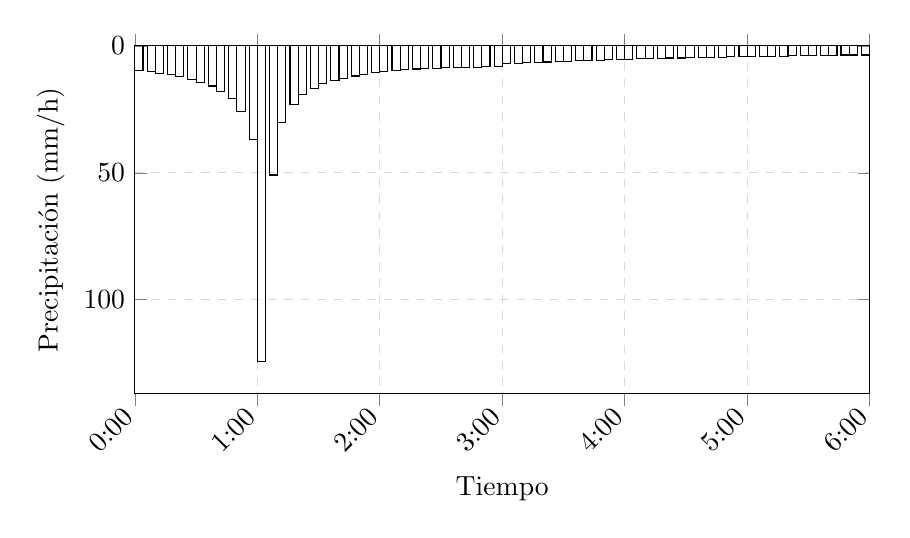
\begin{tikzpicture}
		\begin{axis}[
			width=0.9\textwidth,
			height=6cm,
			xlabel={Tiempo},
			ylabel={Precipitación (mm/h)},
			y dir=reverse,
			ymin=0,
			ymax=137,
			xmin=0,
			xmax=360,
			ybar,
			bar width=4,
			xtick={0, 60, 120, 180, 240, 300, 360},
			xticklabels={0:00, 1:00, 2:00, 3:00, 4:00, 5:00, 6:00},
			xticklabel style={rotate=45, anchor=east},
			grid=major,
			grid style={dashed, gray!30},
			]
			\addplot [
			draw=black,
			fill=none
			]
			coordinates {
				(2, 9.72) (8, 10.20) (12, 10.80) (18, 11.40) (22, 12.24)
				(28, 13.20) (32, 14.40) (38, 15.84) (42, 17.88) (48, 20.88)
				(52, 25.92) (58, 36.96) (62, 124.32) (68, 50.88) (72, 30.12)
				(78, 23.16) (82, 19.32) (88, 16.80) (92, 15.00) (98, 13.68)
				(102, 12.72) (108, 11.88) (112, 11.16) (118, 10.56) (122, 10.08)
				(128, 9.60) (132, 9.36) (138, 9.12) (142, 9.00) (148, 8.76)
				(152, 8.64) (158, 8.40) (162, 8.40) (168, 8.40) (172, 8.16)
				(178, 8.04) (182, 6.96) (188, 6.84) (192, 6.72) (198, 6.48)
				(202, 6.36) (208, 6.24) (212, 6.00) (218, 5.88) (222, 5.76)
				(228, 5.64) (232, 5.52) (238, 5.40) (242, 5.40) (248, 5.16)
				(252, 5.04) (258, 5.04) (262, 4.80) (268, 4.80) (272, 4.68)
				(278, 4.68) (282, 4.56) (288, 4.44) (292, 4.32) (298, 4.32)
				(302, 4.20) (308, 4.20) (312, 4.08) (318, 4.08) (322, 3.96)
				(328, 3.84) (332, 3.84) (338, 3.84) (342, 3.72) (348, 3.60)
				(352, 3.60) (358, 3.60)
			};
		\end{axis}
	\end{tikzpicture}
	\caption{Hietograma - GZ $T_r$=2 años (P=68.6 mm)}
	\label{fig:hyeto_kirpich_gz_Tr2_X125}
\end{figure}
